\section{Gnavere og støttetandede (Artsbestemmeæse \& biologi)}

% ========== TITEL: GNAVERE OG STØTTETANDEDE ==========
\begin{frame}
  \vspace{1.5em}
  \begin{center}
    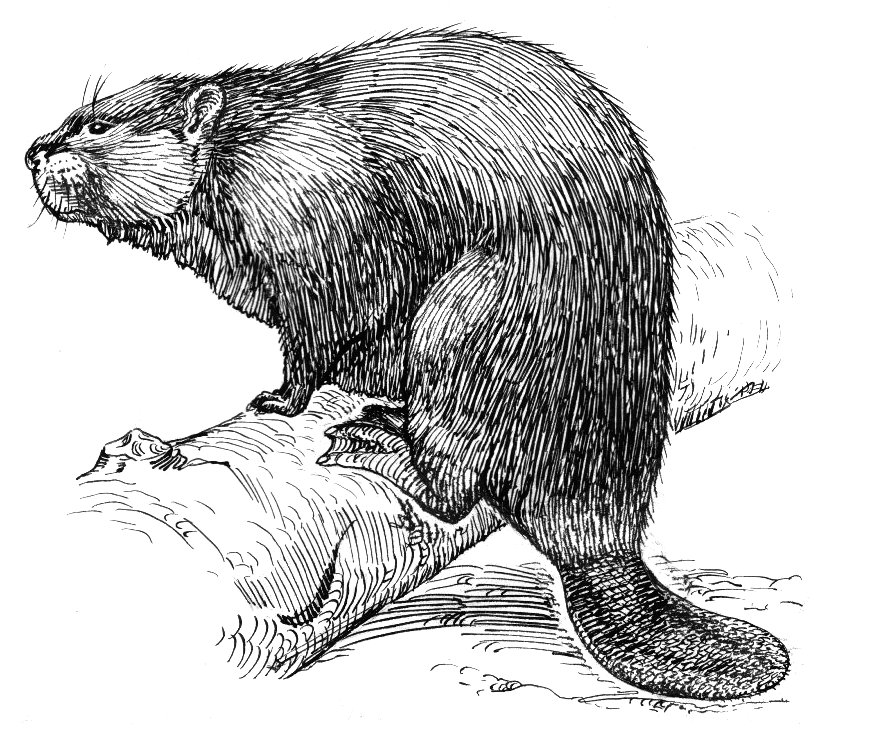
\includegraphics[width=12cm, height=4cm, keepaspectratio]{Billeder/Dyr/Pattedyr/støttetandede/gnaver.jpg}\\[1.2em]
    {\LARGE \textbf{Gnavere og støttetandede}}\\[0.6em]
    
    Artsbestemmelse \& vildtbiologi  \\[0.9em]
    {\tiny\color{gray}
    CC BY 4.0 – kan frit anvendes, også kommercielt. Rettighederne må ikke skærpes.\\[0.05em]
    Udviklet af Aleksander Sønder, OSJAGTTEGN.DK}
  \end{center}
\end{frame}

% ========== HARE ==========
\begin{frame}{%
  \begin{minipage}[c]{0.30\textwidth}
    Hare
  \end{minipage}%
  \hfill
  \begin{minipage}[c]{0.45\textwidth}
    \footnotesize
    \textbf{Jagttid:} 1.\ oktober -- 31.\ januar
  \end{minipage}%
  \hfill
  \begin{minipage}[c]{0.15\textwidth}
    \noindent\raggedleft
    
\includegraphics[width=0.5cm, height=0.5cm, keepaspectratio]{Billeder/Ikoner/star.png}%
    \hspace{0.2em}%
    
\includegraphics[width=0.5cm, height=0.5cm, keepaspectratio]{Billeder/Ikoner/star.png}%
    \hspace{0.2em}%
    
\includegraphics[width=0.5cm, height=0.5cm, keepaspectratio]{Billeder/Ikoner/star.png}
  \end{minipage}%
}
  \vspace{0.25em}
  \begin{columns}[T]
    % --- Venstre kolonne: Tekst ---
    \column{0.45\textwidth}
    \setlength{\parskip}{0.4em}
    \tiny
    \RaggedRight
    \textbf{\textit{Lepus europaeus}} – kendes på de meget lange ører og lange ben. \par
    \textbf{Udseende:}\\
    \quad – Lange ører med sorte spidser \\
    \quad – Gråbrun pels \\
    \quad – Bagben længere end forbenene \par
    \textbf{Levesteder:} Knyttet til det åbne land, men findes også i skovområder. \par
    \textbf{Føde:} Friske skud af græs og urter samt landbrugsafgrøder. Pseudo-drøvtygger. \par
    \textbf{Udbredelse:} Hele landet. \par
    \textbf{Parring/brunst:} Januar--september. \par
    \textbf{Forplantning:}\\
    \quad – \textbf{Kønsmoden:} 1 år \\
    \quad – \textbf{Mono/polygam:} Polygam \\
    \quad – \textbf{Bestandsomsætning:} Hurtig \\
    \quad – \textbf{Kuld:} 2--4 kuld med 2--4 killinger pr.\ kuld \par
    % --- Højre kolonne: Større billede ---
    \column{0.52\textwidth}
    \centering
    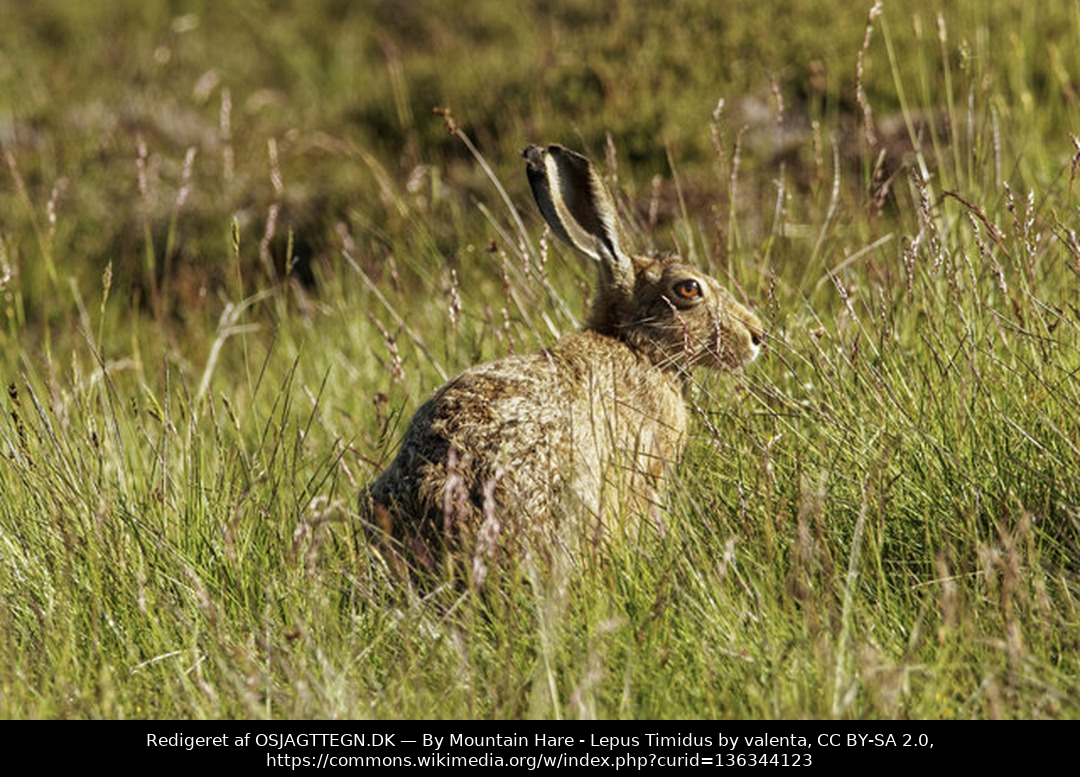
\includegraphics[width=\linewidth, height=7.2cm, keepaspectratio]{Billeder/Dyr/Pattedyr/støttetandede/hare/hare-04.jpg}
  \end{columns}
\end{frame}

% ========== VILDKANIN ==========
\begin{frame}{%
  \begin{minipage}[c]{0.30\textwidth}
    Vildkanin
  \end{minipage}%
  \hfill
  \begin{minipage}[c]{0.45\textwidth}
    \footnotesize
    \textbf{Jagttid:} 1.\ september -- 31.\ januar
  \end{minipage}%
  \hfill
  \begin{minipage}[c]{0.15\textwidth}
    \noindent\raggedleft
    
\includegraphics[width=0.5cm, height=0.5cm, keepaspectratio]{Billeder/Ikoner/star.png}%
    \hspace{0.2em}%
    
\includegraphics[width=0.5cm, height=0.5cm, keepaspectratio]{Billeder/Ikoner/star.png}
  \end{minipage}%
}
  \vspace{0.25em}
  \begin{columns}[T]
    % --- Venstre kolonne: Tekst ---
    \column{0.45\textwidth}
    \setlength{\parskip}{0.4em}
    \tiny
    \RaggedRight
    \textbf{\textit{Oryctolagus cuniculus}} – forholdsvis lange ører, men mere kompakt end haren. \par
    \textbf{Udseende:}\\
    \quad – Benene næsten lige lange \\
    \quad – Brun overside \\
    \quad – Hvid underside \par
    \textbf{Levesteder:} I kolonier under jorden nær åbne arealer. \par
    \textbf{Føde:} Friske skud af græsser og urter samt markafgrøder. Pseudo-drøvtygger. \par
    \textbf{Udbredelse:} Sønderjylland, Fanø, Als, Endelave og Bornholm.
    % --- Højre kolonne: Større billede ---
    \column{0.52\textwidth}
    \centering
    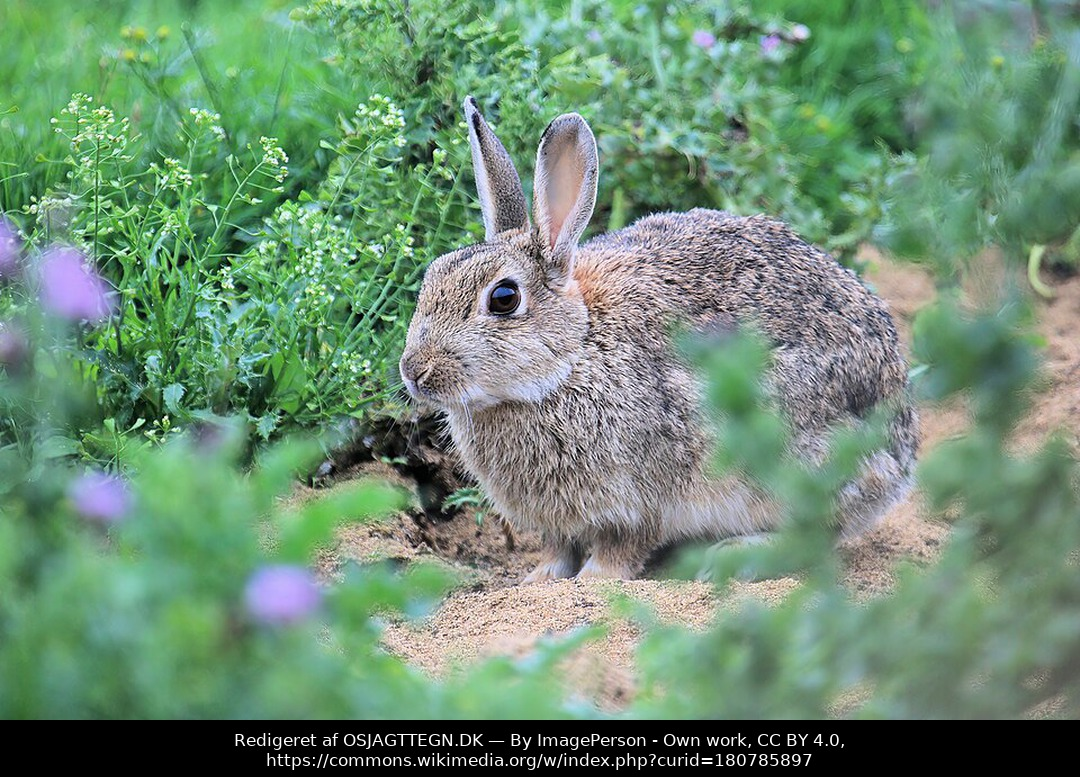
\includegraphics[width=\linewidth, height=7.2cm, keepaspectratio]{Billeder/Dyr/Pattedyr/støttetandede/vildkanin/vildkanin-02.jpg}
  \end{columns}
\end{frame}

% ========== EGERN ==========
\begin{frame}{%
  \begin{minipage}[c]{0.30\textwidth}
    Egern
  \end{minipage}%
  \hfill
  \begin{minipage}[c]{0.45\textwidth}
    \footnotesize
    \textbf{Jagttid:} Ingen jagttid
  \end{minipage}%
  \hfill
  \begin{minipage}[c]{0.15\textwidth}
    \noindent\raggedleft
    
\includegraphics[width=0.5cm, height=0.5cm, keepaspectratio]{Billeder/Ikoner/star.png}
  \end{minipage}%
}
  \vspace{0.25em}
  \begin{columns}[T]
    % --- Venstre kolonne: Tekst ---
    \column{0.45\textwidth}
    \setlength{\parskip}{0.4em}
    \tiny
    \RaggedRight
    \textbf{\textit{Sciurus vulgaris}} – lille gnaver med busket hale. \par
    \textbf{Udseende:}\\
    \quad – Pelsfarven varierer fra rød over brun til næsten sort \\
    \quad – Undersiden er som regel hvid
    % --- Højre kolonne: Større billede ---
    \column{0.52\textwidth}
    \centering
    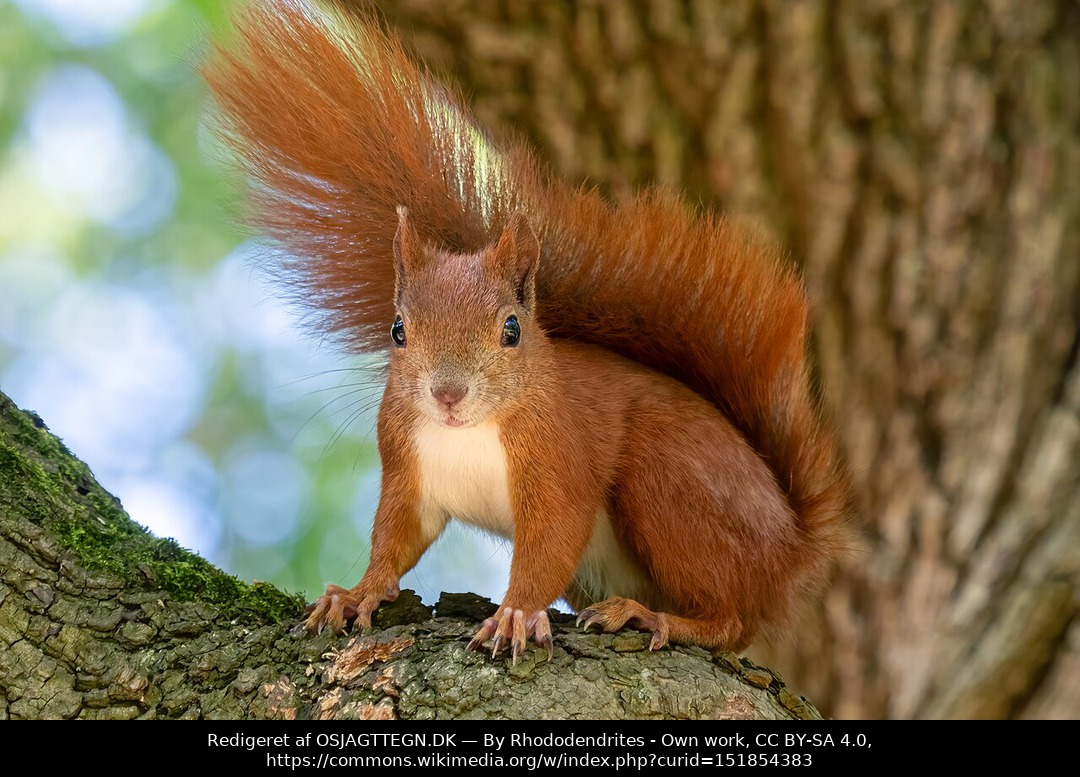
\includegraphics[width=\linewidth, height=7.2cm, keepaspectratio]{Billeder/Dyr/Pattedyr/støttetandede/egern/egern-01.jpg}
  \end{columns}
\end{frame}

% ========== BÆVER ==========
\begin{frame}{%
  \begin{minipage}[c]{0.30\textwidth}
    Bæver
  \end{minipage}%
  \hfill
  \begin{minipage}[c]{0.45\textwidth}
    \footnotesize
    \textbf{Jagttid:} Ingen jagttid
  \end{minipage}%
  \hfill
  \begin{minipage}[c]{0.15\textwidth}
    \noindent\raggedleft
    
\includegraphics[width=0.5cm, height=0.5cm, keepaspectratio]{Billeder/Ikoner/star.png}
  \end{minipage}%
}
  \vspace{0.25em}
  \begin{columns}[T]
    % --- Venstre kolonne: Tekst ---
    \column{0.45\textwidth}
    \setlength{\parskip}{0.4em}
    \tiny
    \RaggedRight
    \textbf{\textit{Castor fiber}} – stor gnaver knyttet til vandløb og søer. \par
    \textbf{Udseende:}\\
    \quad – Ensfarvet pels med lange, stride hår \\
    \quad – Bred, nøgen hale med skællet hud \\
    \quad – Lange, skarpe fortænder
    % --- Højre kolonne: Større billede ---
    \column{0.52\textwidth}
    \centering
    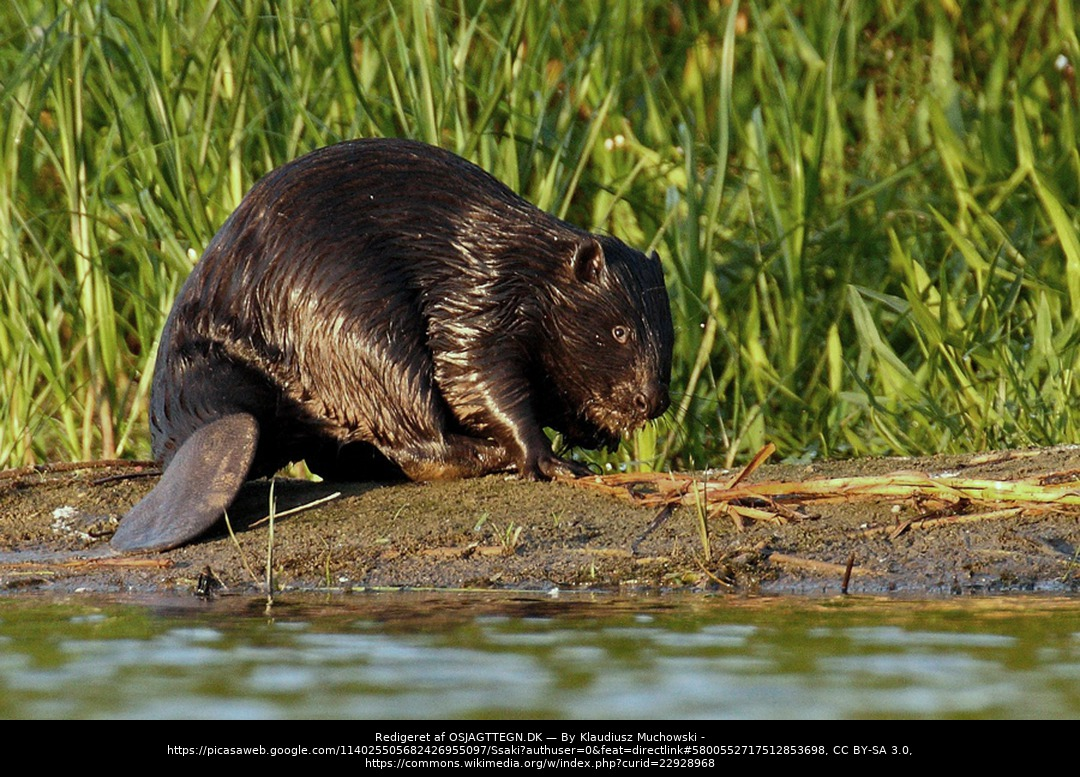
\includegraphics[width=\linewidth, height=7.2cm, keepaspectratio]{Billeder/Dyr/Pattedyr/støttetandede/bæver/baever-01.jpg}
  \end{columns}
\end{frame}

% ========== SUMPBÆVER ==========
\begin{frame}{%
  \begin{minipage}[c]{0.30\textwidth}
    Sumpbæver
  \end{minipage}%
  \hfill
  \begin{minipage}[c]{0.45\textwidth}
    \footnotesize
    \textbf{Jagttid:} Hele året\\
    \textbf{Regulering:} Uden aftale (invasiv)
  \end{minipage}%
  \hfill
  \begin{minipage}[c]{0.15\textwidth}
    \noindent\raggedleft
    
\includegraphics[width=0.5cm, height=0.5cm, keepaspectratio]{Billeder/Ikoner/star.png}
  \end{minipage}%
}
  \vspace{0.25em}
  \begin{columns}[T]
    % --- Venstre kolonne: Tekst ---
    \column{0.45\textwidth}
    \setlength{\parskip}{0.4em}
    \tiny
    \RaggedRight
    \textbf{\textit{Myocastor coypus}} – invasiv gnaver knyttet til vådområder. \par
    \textbf{Udseende:}\\
    \quad – Grov, brunlig pels \\
    \quad – Stort hoved i forhold til kroppen \\
    \quad – Rund, skællet hale med få hår
    % --- Højre kolonne: Større billede ---
    \column{0.52\textwidth}
    \centering
    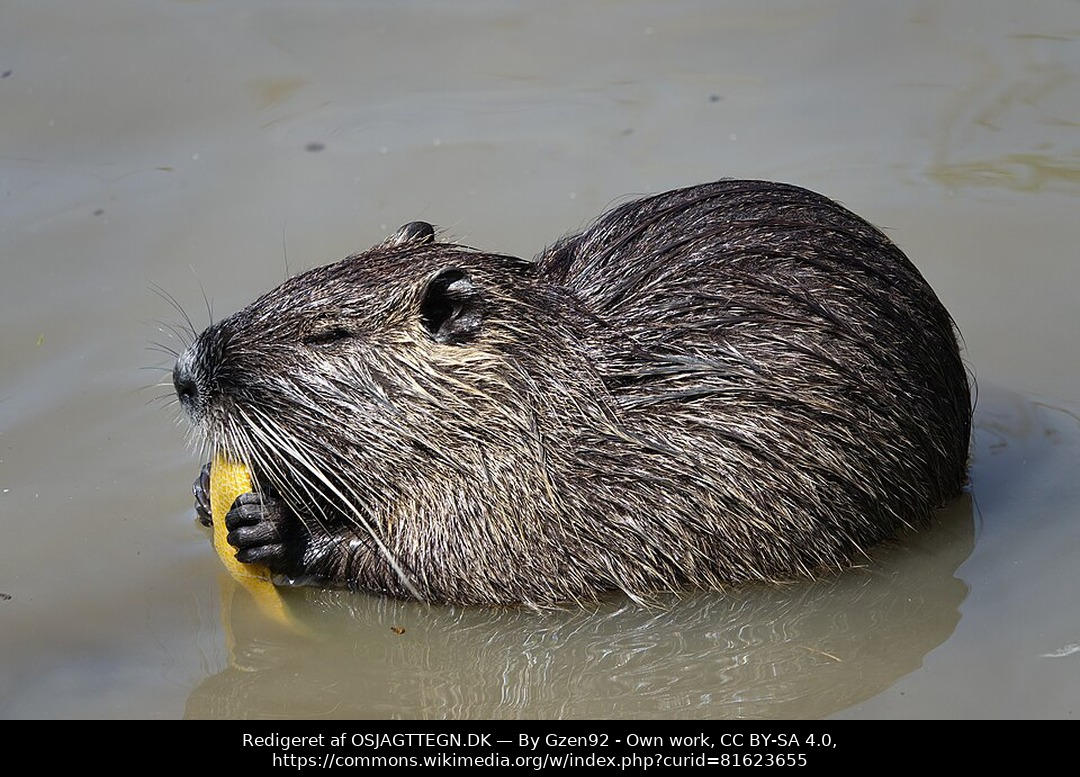
\includegraphics[width=\linewidth, height=7.2cm, keepaspectratio]{Billeder/Dyr/Pattedyr/støttetandede/sumpbæver/sumpbaever-01.jpg}
  \end{columns}
\end{frame}

% ========== BISAMROTTE ==========
\begin{frame}{%
  \begin{minipage}[c]{0.30\textwidth}
    Bisamrotte
  \end{minipage}%
  \hfill
  \begin{minipage}[c]{0.45\textwidth}
    \footnotesize
    \textbf{Jagttid:} Hele året\\
    \textbf{Regulering:} Uden aftale (invasiv)
  \end{minipage}%
  \hfill
  \begin{minipage}[c]{0.15\textwidth}
    \noindent\raggedleft
    
\includegraphics[width=0.5cm, height=0.5cm, keepaspectratio]{Billeder/Ikoner/star.png}
  \end{minipage}%
}
  \vspace{0.25em}
  \begin{columns}[T]
    % --- Venstre kolonne: Tekst ---
    \column{0.45\textwidth}
    \setlength{\parskip}{0.4em}
    \tiny
    \RaggedRight
    \textbf{\textit{Ondatra zibethicus}} – invasiv gnaver knyttet til søer, åer og moser. \par
    \textbf{Udseende:}\\
    \quad – Brunlig og buttet med kort snude \\
    \quad – Hale med skællet hud og få hår
    % --- Højre kolonne: Større billede ---
    \column{0.52\textwidth}
    \centering
    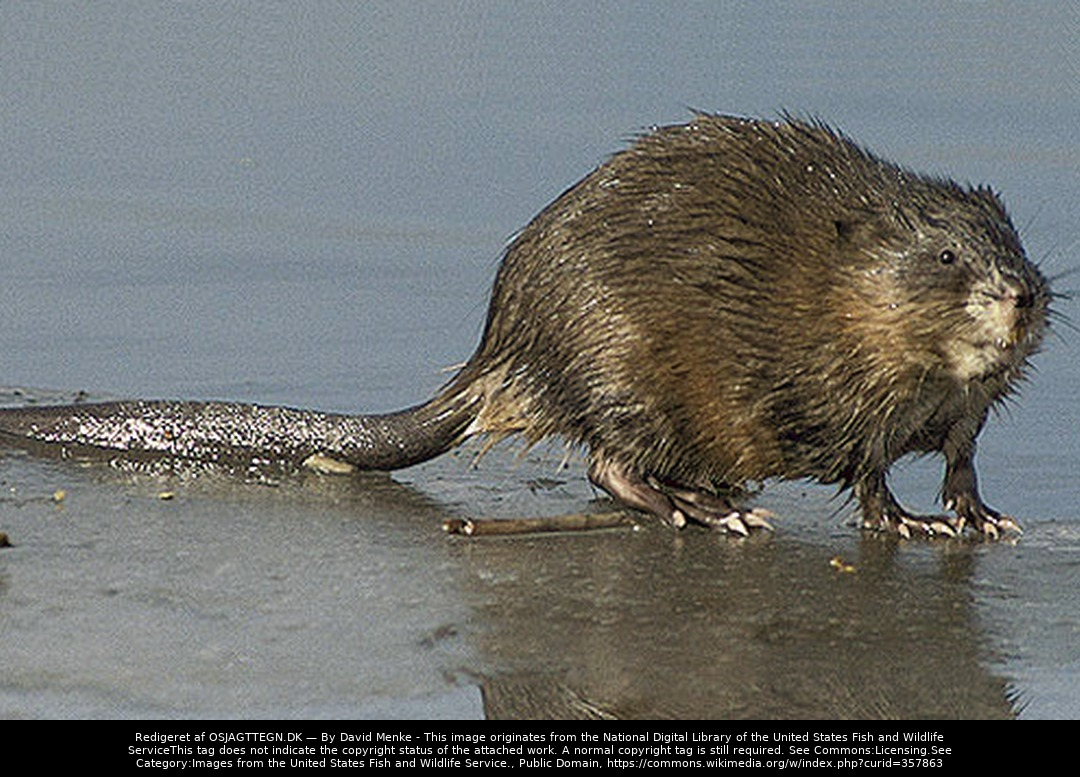
\includegraphics[width=\linewidth, height=7.2cm, keepaspectratio]{Billeder/Dyr/Pattedyr/støttetandede/bisamrotte/bisamrotte-01.jpg}
  \end{columns}
\end{frame}

\begin{frame}
  \vspace{1.8em}
  \begin{center}
    \begin{minipage}{0.22\textwidth}
      \centering
      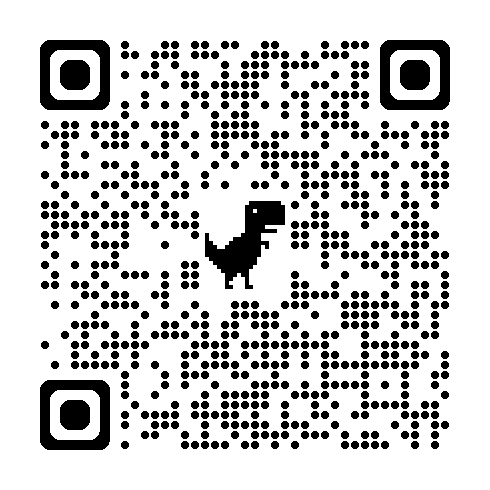
\includegraphics[width=\linewidth]{Billeder/Dyr/Pattedyr/støttetandede/qr_støtte.png}
    \end{minipage}%
    \hspace{0.8em}%
    \begin{minipage}{0.62\textwidth}
      \raggedright
      \Large
      \textbf{Træning i artsbestemmelse af gnavere og støttetandende}\\[0.35em]
      {\large https://osjagttegn.dk/gnavere-og-stoettetandede}
    \end{minipage}
  \end{center}
\end{frame}